% Section 4
% 2021-08-19
% Alessandro Zanatta

\section{Tools comparison}
\label{section:features-comparison}
In this section we will compare tools based on their usability, expressiveness, efficiency, soundness and completeness.

\subsection{Usability}
Let us define usability as the \textbf{easiness of modeling} and specifying security properties of a certain protocol, as well as how easy it is to interpret the \textbf{tool output}, especially when an attack trace is found.

\paragraph{Modeling protocols}
As Verifpal manual also states \cite{VerifpalManual}, ``Verifpal's main aim is to appeal more to real-world practitioners, students and engineers without sacrificing comprehensive formal verification features''. Its language is extremely simple and fast to learn, queries and equational theory, while severely restricted, are usually expressive enough for most cases.
Meanwhile, Proverif and Tamarin both have a steep learning curve as the constructs they are based on can be challenging to grasp at first. Of course, such a statement is hard to prove and has to be partially taken as a personal indication.

Verifpal additionally has a VS-Code extension which enhances the modeling experience with a real-time graph of the protocol being modeled. \Cref{fig:verifpal-protocol-graph} shows the graph for the Anonymous Diffie-Hellman protocol.

\begin{figure}[t]
    \centering
    \makebox[\textwidth][c]{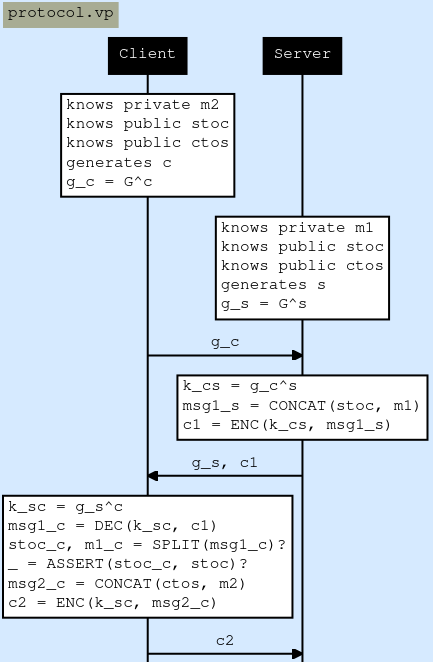
\includegraphics[scale=.45]{verifpal-protocol-graph}}
    \caption{Verifpal's graph using VS-Code plugin.}
    \label{fig:verifpal-protocol-graph}
\end{figure}


\paragraph{Attack traces}
Finally, let us compare tool outputs when an attack trace is found. Verifpal states that its trace is easier to read compared to other tools. Considering a solely textual attack trace in \cref{fig:attack-trace}, it is actually true that Verifpal's trace is easier to understand for an un-experienced user as it indicates what messages were mutated by the adversary.

\begin{figure}[t]
    \centering
    \makebox[\textwidth][c]{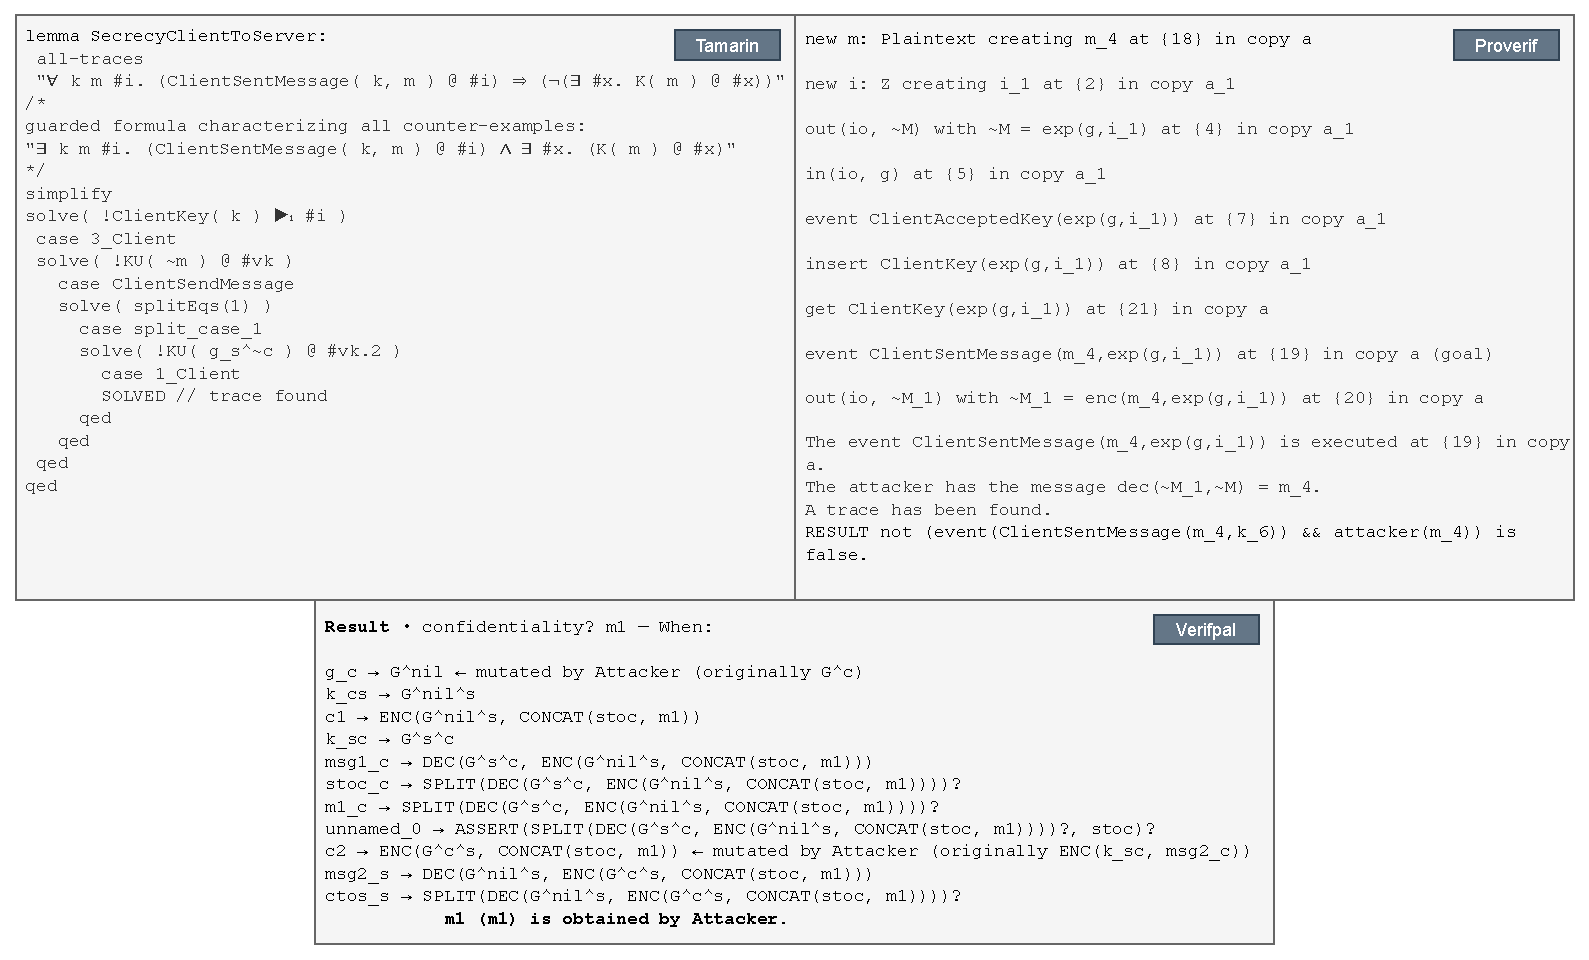
\includegraphics[scale=.65]{attack-trace-comparison}}
    \caption{Textual traces comparison.}
    \label{fig:attack-trace}
\end{figure}

However, Tamarin and Proverif also offer a graph view of the attack, which is far more readable. Tamarin traces, which are offered from its interactive web app, are slightly customizable and can be made more or less verbose. An example is given in \cref{fig:tamarin-trace,fig:proverif-trace}.


\begin{figure}[t]
    \centering
    \makebox[\textwidth][c]{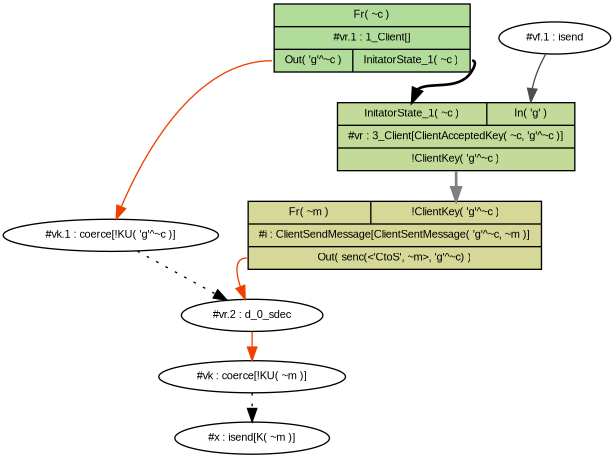
\includegraphics[scale=.75]{tamarin-trace}}
    \caption{Tamarin's attack trace graph view example.}
    \label{fig:tamarin-trace}
\end{figure}
\begin{figure}[t]
    \centering
    \makebox[\textwidth][c]{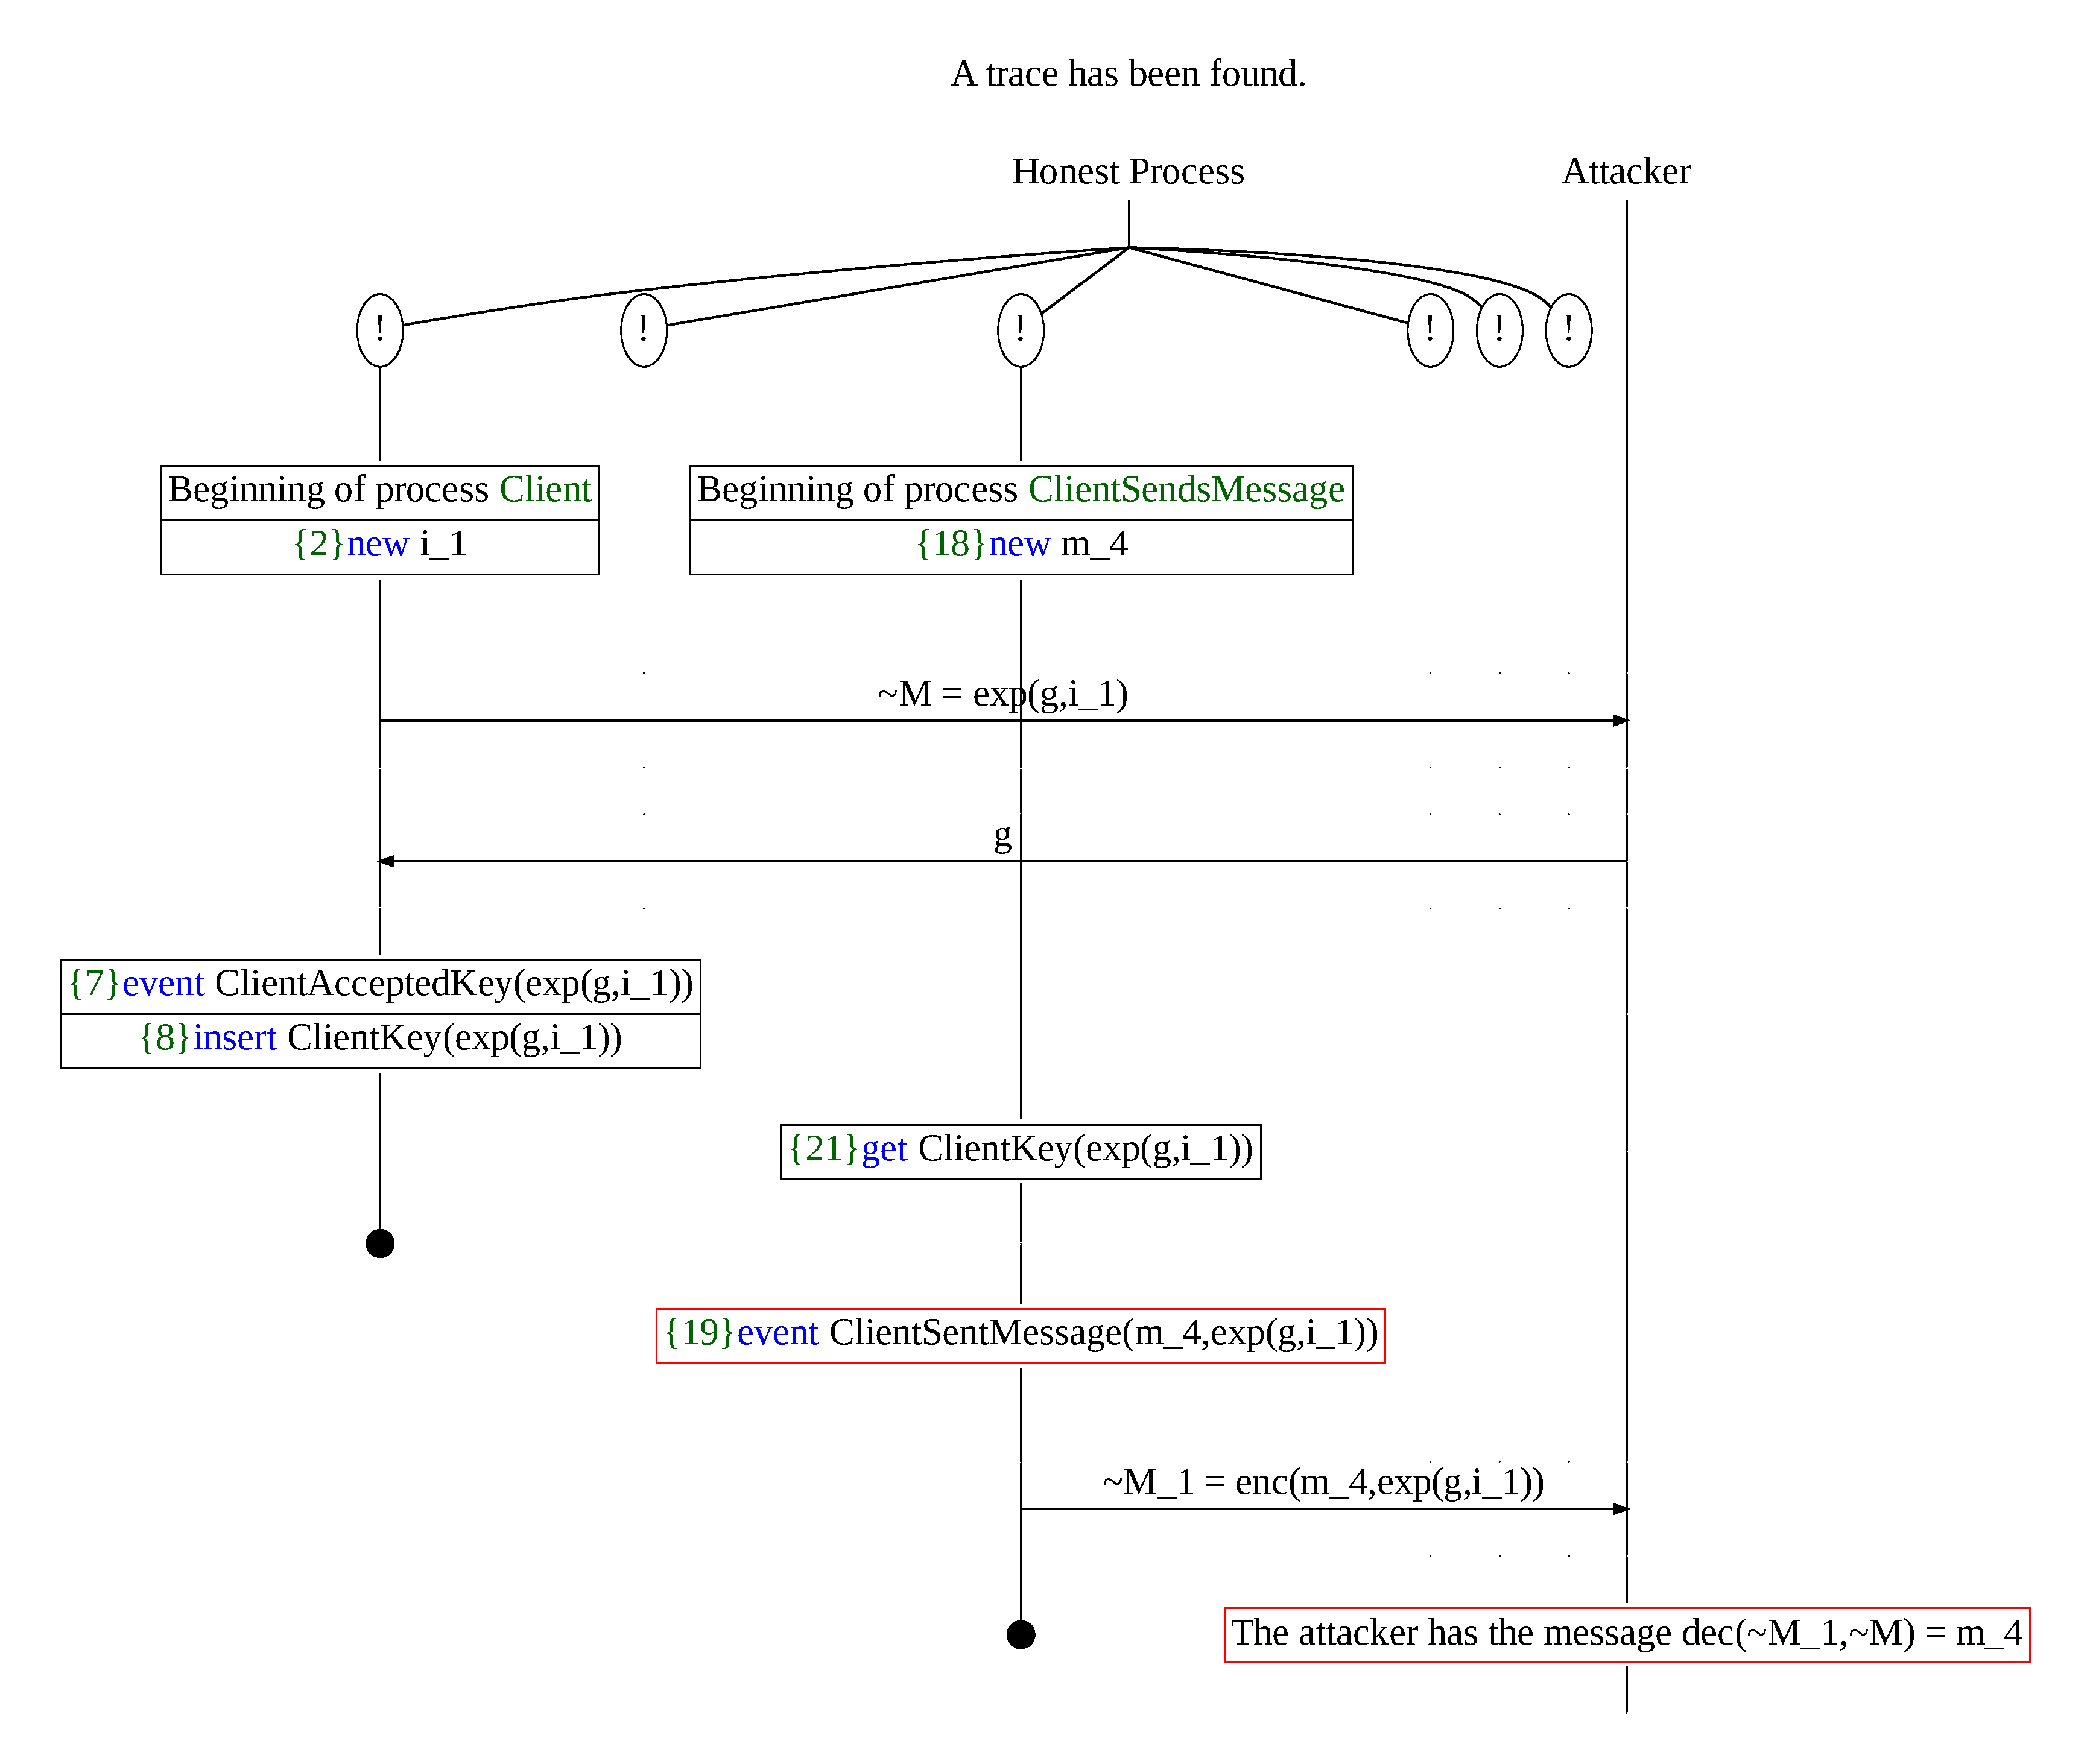
\includegraphics[scale=.3]{proverif-trace}}
    \caption{Proverif's attack trace graph view example.}
    \label{fig:proverif-trace}
\end{figure}


\subsection{Expressiveness}
\Cref{tbl:expressiveness} shows expressiveness of analyzed tools.
All tools assume unbounded sessions. Tamarin's equational theory, with its complex Diffie-Hellman theory (which comprehends 6 equations, including inverse), is way more expressive then the other two tools (in which only commutativity of exponents is possible). Verifpal additionally puts a cap on the number of exponentiations to two, which is not high enough to model Diffie-Hellman with three or more parties \cite{MultipartyDH}.

Proverif support to state is limited to tables, while Tamarin and Verifpal naturally support stateful principals (via different formalisms and syntaxes). Moreover, observational equivalence\footnote{Observational equivalence expresses that two systems appear the same to the environment.} is not supported by Verifpal (which only supports equivalence of terms), but it supports linkability\footnote{Verifpal uses the following definition \cite{VerifpalFoundations}: ``for two
    observed values, the adversary cannot distinguish between a protocol execution in
    which they belong to the same user and a protocol execution in which they belong to
    two different users''.}.

\begin{table}[!ht]
    \renewcommand{\arraystretch}{1.5}
    \setlength\arrayrulewidth{1pt}
    \rowcolors{2}{gray!25}{white}
    \makebox[\textwidth][c]{
        \scalebox{0.9}{
            \begin{tabular}{c|ccccc}
                \multicolumn{1}{l|}{} & \textbf{Unbounded} & \textbf{Equational theory} & \textbf{State} & \textbf{Obs. Equiv.} & \textbf{Linkability} \\ \hline
                \textbf{Tamarin}      & \fullcirc          & \fullcirc                  & \fullcirc      & \fullcirc            & \emptycirc           \\
                \textbf{Proverif}     & \fullcirc          & \halfcirc                  & \halfcirc      & \fullcirc            & \emptycirc           \\
                \textbf{Verifpal}     & \fullcirc          & \halfcirc                  & \fullcirc      & \emptycirc           & \fullcirc
            \end{tabular}
        }
    }
    \caption{Expressiveness of tools.}
    \label{tbl:expressiveness}
\end{table}

\subsection{Efficiency}
\Cref{tab:DH,tab:NSPK} shows three metrics for each tool and protocol version: peak memory usage (in kb), elapsed time since start and cpu time (as system load).

Measures were taken using hyperfine \cite{hyperfine} and time \cite{time}.

As it can be seen, Tamarin memory usage is about 3 to 5 times the one of Proverif and Verifpal, while time to complete proofs is about one to two orders of magnitude higher. We can also notice that Proverif is a single-threaded prover\footnote{As cpu time is always $\leq 1$, this means that Proverif is using at most a single core.}, while Tamarin and Verifpal are extensively using all available cores\footnote{The benchmark system has a total of 4 cores.}.


\begin{table}[!ht]
\caption{Comparison table for Diffie-Hellman.}
\label{tab:DH}
\setlength\arrayrulewidth{1pt}
\rowcolors{2}{gray!25}{white}
\makebox[\textwidth][c]{
    \scalebox{0.9}{
    \begin{tabular}{c|ccc|ccc|ccc|l}
    \cline{2-10}
    \multicolumn{1}{l|}{} & \multicolumn{3}{c|}{\textbf{Peak memory size (kb)}} & \multicolumn{3}{c|}{\textbf{Time (s)}} & \multicolumn{3}{c|}{\textbf{CPU time}} &  \\ \cline{2-10}
    \multicolumn{1}{l|}{}                    & Tamarin & Verifpal & Proverif & Tamarin & Verifpal & Proverif & Tamarin & Verifpal & Proverif & \\ \hline
    \multicolumn{1}{c|}{Mean}      & 52445 & 11480 & 10639 & 1136 & 13  & 44  & 3.52 & 2.08 & 0.98 & \multicolumn{1}{c}{} \\ \cline{1-10}
    \multicolumn{1}{c|}{Deviation} & 2541  & 244   & 108   & 106  & 1   & 1   & 0.06 & 0.12 & 0.02 & \multicolumn{1}{c}{} \\ \cline{1-10}
    \multicolumn{1}{c|}{Median}    & 52120 & 11464 & 10616 & 1125 & 12  & 44  & 3.52 & 2.08 & 0.97 & \multicolumn{1}{c}{\parbox[t]{1em}{\multirow{-3}{*}{\rotatebox[origin=c]{90}{\textbf{Anon}}}}} \\ \hline
    
    \multicolumn{1}{c|}{Mean}      & 39731 & 13112 & 10623 & 841  & 67  & 34  & 3.38 & 3.24 & 0.98 & \multicolumn{1}{c}{} \\ \cline{1-10}
    \multicolumn{1}{c|}{Deviation} & 1824  & 257   & 110   & 106  & 7   & 0   & 0.04 & 0.06 & 0.02 & \multicolumn{1}{c}{} \\ \cline{1-10}
    \multicolumn{1}{c|}{Median}    & 39742 & 13008 & 10604 & 814  & 72  & 34  & 3.38 & 3.25 & 0.97 & \multicolumn{1}{c}{\parbox[t]{1em}{\multirow{-3}{*}{\rotatebox[origin=c]{90}{\textbf{Eph}}}}} \\ \hline

    \multicolumn{1}{c|}{Mean}      & 44273 & 13098 & 11112 & 1312 & 75 & 81 & 3.47 & 3.14 & 0.98 & \multicolumn{1}{c}{} \\ \cline{1-10}
    \multicolumn{1}{c|}{Deviation} & 1518  & 250   & 112   & 201  & 8  & 1  & 0.04 & 0.10 & 0.01 & \multicolumn{1}{c}{} \\ \cline{1-10}
    \multicolumn{1}{c|}{Median}    & 43914 & 12994 & 11092 & 1319 & 80 & 81 & 3.48 & 3.16 & 0.98 & \multicolumn{1}{c}{\parbox[t]{1em}{\multirow{-3}{*}{\rotatebox[origin=c]{90}{\textbf{PFS}}}}} \\
    \end{tabular}
    }
}
\end{table}

\begin{table}[!ht]
\caption{Comparison table for Needham-Schroeder Public Key.}
\label{tab:NSPK}
\makebox[\textwidth][c]{
    \begin{tabular}{c|c|c|c|c|c|c|c|c|c|l}
    \cline{2-10}
    \multicolumn{1}{l|}{} & \multicolumn{3}{c|}{\textbf{Peak memory size (kb)}} & \multicolumn{3}{c|}{\textbf{Time (s)}} & \multicolumn{3}{c|}{\textbf{CPU time}} &  \\ \cline{2-10}
    \multicolumn{1}{l|}{}                    & Tamarin & Verifpal & Proverif & Tamarin & Verifpal & Proverif & Tamarin & Verifpal & Proverif & \\ \hline
    \multicolumn{1}{|c|}{Mean} & 59803 & 13286 & 11106 & 3336 & 40 & 86 & 3.70 & 2.05    & 0.99 & \multicolumn{1}{l|}{\parbox[t]{1em}{\multirow{3}{*}{\rotatebox[origin=c]{90}{\textbf{Flawed}}}}} \\ \cline{1-10}
    \multicolumn{1}{|c|}{Deviation} & 2860 & 317 & 107 & 188 & 4 & 1 & 0.05 & 0.05 & 0.01 & \multicolumn{1}{l|}{} \\ \cline{1-10}
    \multicolumn{1}{|c|}{Median}    & 59498 & 13224 & 11088 & 3345 & 40 & 86 & 3.70 & 2.05 & 0.98 & \multicolumn{1}{l|}{} \\ \specialrule{.2em}{0em}{0em}

    \multicolumn{1}{|c|}{Mean}      & 53217 & NA & 10698 & 1929 & NA & 69 & 3.63 & NA    & 0.99 & \multicolumn{1}{l|}{\parbox[t]{1em}{\multirow{3}{*}{\rotatebox[origin=c]{90}{\textbf{Fixed}}}}} \\ \cline{1-10}
    \multicolumn{1}{|c|}{Deviation} & 2802 & NA & 109 & 164 & NA & 1 & 0.05 & NA & 0.01 & \multicolumn{1}{l|}{} \\ \cline{1-10}
    \multicolumn{1}{|c|}{Median}    & 53400 & NA & 10672 & 1929 & NA & 68 & 3.63 & NA    & 0.98 & \multicolumn{1}{l|}{} \\ \hline
    
    \end{tabular}
}
\end{table}

\newpage
\subsection{Soundness and completeness}

Let us define, in an informal way, what soundness and completeness of formal verification tools means. Please refer to \cite{Furer89oncompleteness} for a more detailed description.

\textbf{Soundness} means that any statement that can be proven is valid (i.e. there is no proof for a false statement).

\textbf{Completeness} means that the proof system is powerful enough to prove any valid statement.

Soundness and completeness of analyzed tools is summarized in \cref{tbl:sound-complete}.
Tamarin is both sound and complete, meaning that it will always give the correct answer to queries, assuming termination. Proverif, being sound but not complete, may be unable to prove some statements and terminate with an inconclusive result. Finally, Verifpal has no formal guarantee at all, but evidence has shown that in real-case scenarios the tool performs correctly.

\begin{table}[!ht]
    \centering
    \setlength\arrayrulewidth{1pt}
    \renewcommand{\arraystretch}{1.4}
    \rowcolors{2}{gray!25}{white}
    \scalebox{0.9}{
        \begin{tabular}{c|cc}
            \multicolumn{1}{l|}{}   & \textbf{Soundness} & \textbf{Completeness} \\ \hline
            \textbf{Tamarin prover} & \cmark             & \cmark                \\
            \textbf{Proverif}       & \cmark             & \xmark                \\
            \textbf{Verifpal}       & \xmark             & \xmark
        \end{tabular}
    }
    \caption{Soundness and completeness of Tamarin, Proverif and Verifpal.}
    \label{tbl:sound-complete}
\end{table}

\comment{
Tamarin
Pros:
- More expressive formulas for security properties
- Sound and complete
- Can prove observational equivalence
- Possibility of manually guiding the proof when heuristics fail to do so automagically
- Can model many algebraic properties of groups for DH key exchanges (comes with higher computational cost!)
- Can model xor and elliptic curve operations
- Supports user defined equational theories
- More flexibility on post compromise properties using timepoints, but lemmas become more verbose
- IS SOUND AND COMPLETE
Cons:
- Probably harder to model
- Slower (do benchmarks!!)


Proverif
Pros:
- Long history
- Can prove observational equivalence
- Supports user defined equational theories
Cons:
- Uses an old-style syntax
- CANNOT model many algebraic properties of groups for DH key exchanges (only commutativity)
- IS SOUND, BUT NOT COMPLETE


Verifpal
Pros:
- Very simple to use (both model specification and queries), while being expressive enough for most use cases (not for 3 parties DH)
- Possibility to translate to proverif/coq (even though its limited)
- Very intuitive language
Cons:
- There may be queries that CANNOT be expressed (try finding a counterexample!)
- CANNOT prove observational equivalence
- It's very recent, still in beta
- CANNOT model many algebraic properties of groups for DH key exchanges (only commutativity ???)
- does NOT support user-defined equational theories
- Does NOT allow to express injectivity
- Does NOT produce a graphical representation of traces automatically
- Feels VERY different from other tools
- Impossible to model 3 parties DH exchange, for example

- IS NOR SOUND NOR COMPLETE


}